\input{../../resources/assignment-head.tex}

\title{hw3-circuits-and-logic}
\date{Due: 02/12/26 at 5pm (late submission until 8am next morning)}
\begin{document}
\maketitle
\thispagestyle{fancy}

{\bf In this assignment}, you will consider how circuits and logic can be used to represent
mathematical claims. You will use propositional operators
to express and evaluate these claims.  You will analyze statements and determine if they are true or false using valid proof strategies.

{\bf Relevant class material}: Week 3, 4, and 5.

You will submit this assignment via Gradescope
(\href{https://www.gradescope.com}{https://www.gradescope.com}) 
in the assignment called ``hw3-circuits-and-logic''.

\instructions

{\bf Assigned questions}

\begin{enumerate}[labelindent=0pt, leftmargin=0pt]  
        \item Circuits. 
        \begin{enumerate}
            \item Consider the circuit below with inputs $x$ and $y$. 
            Can one of the AND gates be exchanged with the OR gate without changing the input-output table of the circuit?
            If so, write 
            out the input-output table that results, and briefly explain why 
            this exchange works. If not,
            explain why not with reference to the definitions
            of the logic gates.            
        \begin{center}
            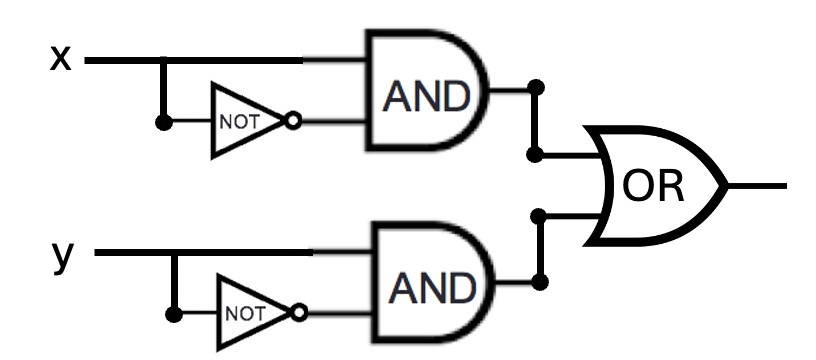
\includegraphics[width=2in]{../../files/circuits-hw3.png}
        \end{center}

        \item Is there a way to fill in the blank portion of 
        the two logic circuits below *with the same gates connected in the same way*
        so that the resulting circuits have the same 
        input-output value *even though* one uses an OR gate at the end and the other 
        uses an XOR gate? If so, design the circuit that would be used, write 
        out the input-output table that results, and briefly explain why your 
        design works. If not, explain why not with reference to the definitions
        of the logic gates.
        \begin{multicols}{2}
            \begin{center}
                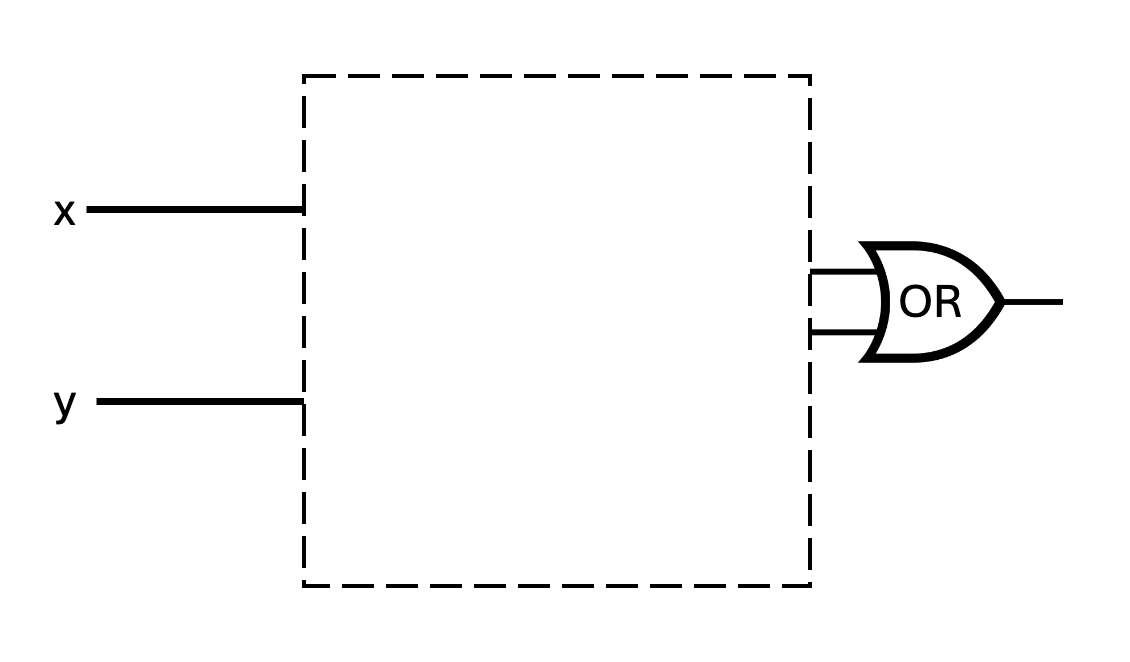
\includegraphics[width=2in]{../../files/circuit-blank-or-hw3.png}
            \end{center}
     
            \begin{center}
                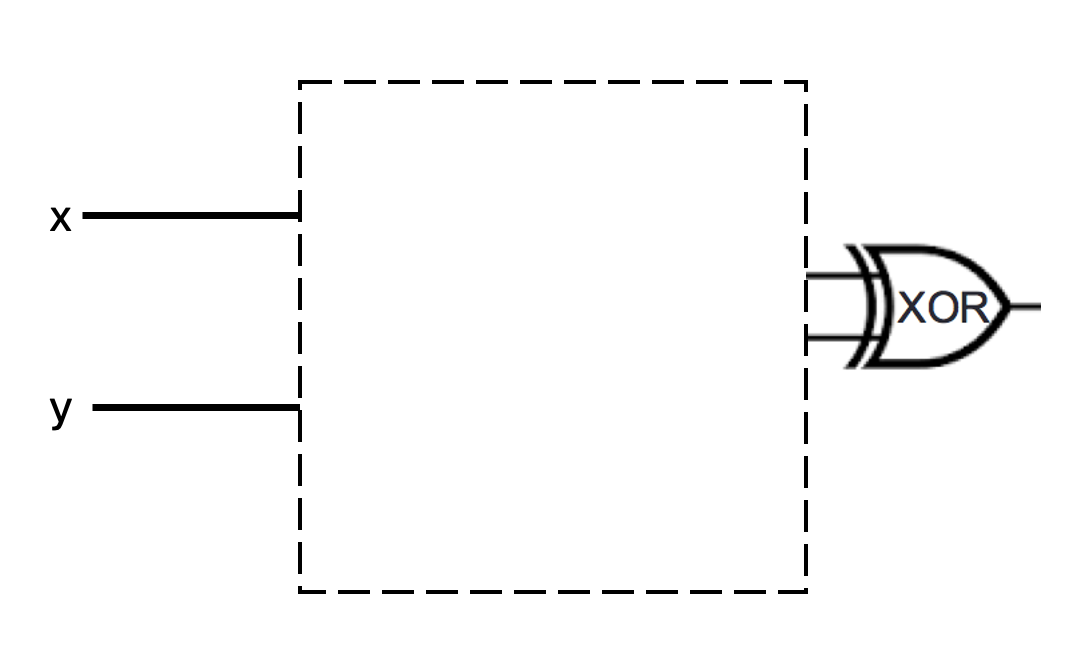
\includegraphics[width=2in]{../../files/circuit-blank-xor-hw3.png}
            \end{center}
        \end{multicols}

    \end{enumerate}

    \item Compound propositions. The set of strings of length $4$ whose characters are $0$s or $1$s is
        the result of four successive set-wise concatenations: $\{0,1\} \circ \{0,1\} \circ \{0,1\}\circ \{0,1\}$. Let's call
        this set $X_4$. Consider the function $f: X_4 \to X_4$ defined by
        $$ f(x) = 
        \begin{cases} 
            y &\text{when $(x)_{2,4} < 15$ and $(y)_{2,4} = (x)_{2,4} + 1$}\\
            1111 &\text{when $x = 1111$}
        \end{cases}$$
        for each $x \in X_4$. In other words, we can describe the function as: $f$ takes a string, interprets it as the binary fixed-width $4$
        expansion of an integer, and then adds $1$ to that integer (unless $x$ is already representing
        the greatest integer that can be represented in binary fixed-width $4$) and outputs the binary 
        fixed-width $4$ expansion of the result.
        \begin{enumerate} 
        \item Fill in the blanks in the following input-output definition table 
        with four inputs $x_3$, $x_2$, $x_1$, $x_0$ and four outputs $y_3$, $y_2$, $y_1$, $y_0$
        so that $f(x_3x_2x_1x_0) = y_3y_2y_1y_0$. Remember to explain all your answers.
        
        \begin{center}
        \begin{tabular}{cccc|cccc}
        $x_3$ & $x_2$ & $x_1$ & $x_0$ & $y_3$ & $y_2$ & $y_1$ & $y_0$\\
        \hline
        $1$ & $1$ & $1$ & $1$ & $1$ & $1$ & BLANK1 & $1$\\
        $1$ & $1$ & $1$ & $0$ & $1$ & $1$ & $1$ & $1$\\
        $1$ & $1$ & $0$ & $1$ & $1$ & BLANK2 & $1$ & $0$\\
        $1$ & $1$ & $0$ & $0$ & $1$ & $1$ & $0$ & $1$\\
        $1$ & $0$ & $1$ & $1$ & $1$ & $1$ & $0$ & $0$\\
        $1$ & $0$ & $1$ & $0$ & $1$ & $0$ & $1$ & $1$\\
        $1$ & $0$ & $0$ & $1$ & $1$ & $0$ & $1$ & $0$\\
        $1$ & $0$ & $0$ & $0$ & BLANK3& $0$ & $0$ & $1$\\
        $0$ & $1$ & $1$ & $1$ & $1$ & $0$ & $0$ & $0$\\
        $0$ & $1$ & $1$ & $0$ & $0$ & $1$ & $1$ & BLANK4\\
        $0$ & $1$ & $0$ & $1$ & $0$ & $1$ & $1$ & BLANK5\\
        $0$ & $1$ & $0$ & $0$ & $0$ & $1$ & $0$ & $1$\\
        $0$ & $0$ & $1$ & $1$ & $0$ & $1$ & $0$ & $0$\\
        $0$ & $0$ & $1$ & $0$ & $0$ & $0$ & $1$ & $1$\\
        $0$ & $0$ & $0$ & $1$ & $0$ & $0$ & $1$ & $0$\\
        $0$ & $0$ & $0$ & $0$ & BLANK6 & $0$ & $0$ & $1$\\
        \end{tabular}
        \end{center}
  
        \item
        Construct an expression (as a compound proposition) for each of $y_0$, $y_1$, $y_2$, and $y_3$ in terms of the inputs 
        $x_3, x_2, x_1, x_0$. Justify your expression by referring to the definition of the logic 
        gates XOR, AND, OR, NOT and the definition of the function $f$. Hint: our work on the half-adder might 
        be helpful.
       
        \item Draw a combinatorial circuit corresponding to two (or more) of these (output) compound propositions.
        Remember that the symbols for the inputs will be on the left-hand-side and 
        the symbol for the outputs $y_0$ and/or $y_1$ and/or $y_2$ and/or $y_3$ will be on the right-hand side. Use gates (draw the appropriate
        shapes and add labels for clarity) and wires to connect the inputs appropriately to give the output.

        \end{enumerate}

        \item Logical Equivalence. Imagine a friend suggests the following argument to you: ``The compound proposition
        \[
        (x \lor y) \land z
        \]
        is logically equivalent to 
        \[
        x \lor (y \land z)
        \]
        because I can transform one to the other using the following sequence of logical equivalences: 
        \[
           (x \lor y) \land z \equiv
           (x \lor (y \land y)) \land z \equiv
           x \lor ( (y \lor y) \land z) \equiv x \lor (y \land z) 
        \]
        because $y$ is logically equivalent to both $y \land y$ and to $y \lor y$".
        
        \begin{enumerate}
        \item Prove to your friend that they made a mistake by giving a truth
        assignment to the propositional variables $x,y,z$ so that 
        the two compound propositions 
        $ (x \lor y) \land z$ and $ x \lor (y \land z)$ have different truth values.
        Justify your choice by evaluating these compound propositions using the definitions of the logical connectives 
        and include enough intermediate steps so that a student in CSE 20 who may be 
        struggling with the material can still follow along with your reasoning.
        
        \item
        Help your friend find the problem in their argument by pointing out which step(s) were incorrect and why.
        
        \item Give {\bf three} different compound propositions
        that are actually logically equivalent to (and not the same as)
        \[
            (x \lor y) \land z
        \]
        Justify each one of these logical equivalences either by applying a sequence of logical equivalences
        or using a truth table.  Notice that you can use other logical operators (e.g. $\lnot, \lor, \land, \oplus, \to, 
        \leftrightarrow$) 
        when constructing your compound propositions.
     
        {\it Bonus; not for credit (do not hand in)}: How would you translate each of the equivalent compound
        propositions in English? Does doing so help illustrate why they are equivalent?
        \end{enumerate}
        
    \vfill
    \newpage 
    \item  Evaluating predicates. Consider the following predicates, each of which has 
    as its domain the set of all bitstrings whose leftmost bit is $1$
    
    $E(x)$ is $T$ exactly when $(x)_{2}$ is even, and is $F$ otherwise
    
    $L(x)$ is $T$ exactly when $(x)_2 < 15$, and is $F$ otherwise
    
    $M(x)$ is $T$ exactly when $(x)_2 > 2$ and is $F$ otherwise.
    
    
    \rule{0.5\textwidth}{.4pt}
    
    {\it Sample response that can be used as reference for the detail expected 
    in your answer:} To prove that the statement $$\forall x ~L(x)$$ is false, we can use 
    the counterexample $x = 1111$, which is a bitstring whose leftmost bit is $1$ (so is in the domain).
    Applying the definition of $L(x)$, since $(1111)_2 = 1 \cdot 2^3 + 1\cdot 2^2 + 1 \cdot 2^1 + 1 \cdot 2^0 = 8 + 4+2+1 = 15$
    which is not (strictly) less than $15$, we have that $L(1111) = F$ and so the universal statement is false.
    
    
    \rule{0.5\textwidth}{.4pt}
    

    \begin{enumerate}
    \item Use a counterexample to prove that the statement
    \[
    \forall x ( ~L(x) \to E(x)~)
    \]
    is false.   Your proof needs to include references to the relevant definitions.

    
    \item Use a witness to prove that the statement
    \[
    \exists x (~L(x) \land M(x) ~)
    \]
    is true.  Your proof needs to include references to the relevant definitions.

    
    \item Translate each of the statements in the previous two
    parts to English.
    \end{enumerate}

        
    \vfill
    \newpage 
    \item Set properties. Let $W = \mathcal{P}(\{1,2,3,4,5\})$. 


    \rule{0.5\textwidth}{.4pt}
    
    {\it Sample response that can be used as reference for the detail expected 
    in your answer for parts (a) and (b) below:} 
    
    To give an example element in the set 
    $\{ X \in W ~|~ 1 \in X \} \cap \{ X \in W ~|~  2 \in X \}$,
    consider $\{ 1,2\}$. To prove that this is in the set, by definition of intersection, we need to show
    that $\{1,2\} \in \{ X \in W ~|~ 1 \in X \}$ and that $\{1,2\} \in \{ X \in W ~|~ 2 \in X \}$.
    \begin{itemize}
    \item By set builder notation, elements in $\{ X \in W ~|~ 1 \in X \}$ have to be elements of $W$ which have $1$ as an element. By definition of power set, elements of $W$ are subsets of $\{1,2,3,4,5\}$. Since
    each element in $\{1,2\}$ is an element of $\{1,2,3,4,5\}$, $\{1,2\}$ is a subset of $\{1,2,3,4,5\}$ 
    and hence is an element of $W$. Also, by roster method, $1 \in \{1,2\}$. Thus, $\{1,2\}$ satisfies the 
    conditions for membership in $\{ X \in W ~|~ 1 \in X \}$.
    \item Similarly, by set builder notation, elements in $\{ X \in W ~|~ 2 \in X \}$ have to be elements of $W$ 
    which have $2$ as an element. 
    By definition of power set, elements of $W$ are subsets of $\{1,2,3,4,5\}$. Since
    each element in $\{1,2\}$ is an element of $\{1,2,3,4,5\}$, $\{1,2\}$ is a subset of $\{1,2,3,4,5\}$ 
    and hence is an element of $W$. Also, by roster method, $2 \in \{1,2\}$. Thus, $\{1,2\}$ satisfies the 
    conditions for membership in $\{ X \in W ~|~ 2 \in X \}$.
    \end{itemize}
    
    \rule{0.5\textwidth}{.4pt}
    
    
    \begin{enumerate}
    \item Give two (different) example elements in 
    \[
    W \times \mathcal{P}(W)
    \]
    Justify your examples by explanations that include references to the relevant definitions.
    
    \item Give one example element in 
    \[
    \{ X \in W \mid (1 \in X) \land (X \cap \{3,4\} = \emptyset) \}
    \]
    Justify your example by explanations that include references to the relevant definitions.
    
    \item Consider the following statement and attempted proof:
    
    
    $$\forall A \in W \, \forall B \in W ~\left(~((A \cap B) \subseteq A) \to (A \subseteq B)~\right)$$
    
    \begin{quote}
    (1) Towards a universal generalization argument, {\bf choose arbitrary} $A \in W, B \in W$ .
    
    (2) We need {\bf to show} $((A \cap B) \subseteq A) \to (A \subseteq B)$.
    
    (3) Towards a proof of the conditional by the contrapositive, {\bf assume} $A \subseteq B$, and we need {\bf to show} 
    that $(A \cap B) \subseteq A$.
    
    (4) By definition of subset inclusion, this means we need {\bf to show} 
    $\forall x ~( x \in A \cap B \to  x \in A  ~)$.
    
    (5) Towards a universal generalization, {\bf choose arbitrary} $x$; we need {\bf to show} that \\
    $x \in A \cap B \to x \in A$.
    
    (6) Towards a direct proof, {\bf assume} $x \in A \cap B$, and we need {\bf to show } $x \in A$.
    
    (7) By definition of set intersection and set builder notation, we have that $x \in A \land x \in B$.
    
    (8) By the definition of conjunction, $x \in A$, which is  what we needed to show. QED
    \end{quote}
    
    Demonstrate that this attempted proof is invalid by providing
    and justifying a {\bf counterexample} (disproving the statement).
    Then, explain why this attempted proof is 
    invalid by identifying in which step a definition or proof strategy is used incorrectly, and describing how the 
    definition or proof strategy was misused.

\end{enumerate}

\end{enumerate}
\vfill
\newpage
In your proofs and disproofs of statements above, justify each  step
by reference to  a component of the  following proof  strategies
we  have discussed so far, and/or to relevant definitions and calculations.

\begin{itemize}
    \item A counterexample can be used to prove that  $\forall x P(x)$ is {\bf false}.
    \item  A witness can be used  to  prove that  $\exists x P(x)$ is {\bf true}.
    \item {\bf Proof of universal by exhaustion}: To prove that $\forall x \, P(x)$
is true when $P$ has a finite domain, evaluate the predicate at {\bf each} domain element to confirm that it is always T.
    \item  {\bf Proof by universal generalization}: To prove that $\forall x \, P(x)$
is true, we can take an arbitrary element $e$ from the domain and show that $P(e)$ is true, without making any assumptions about $e$ other than that it comes from the domain.
    \item To  prove  that $\exists x P(x)$ is {\bf false}, write the universal statement that is logically equivalent to its negation and then prove it true using universal generalization.
    \item {\bf Strategies for conjunction}: To prove that $p \land q$ is true, have two subgoals: subgoal (1) prove $p$ 
is  true; and, subgoal (2) prove $q$ is true. To prove that $p \land q$ is false, it's enough to prove that $p$ is false.
 To prove that $p \land q$ is false, it's enough to prove that $q$ is false.
    \item {\bf Proof of Conditional by Direct Proof}: To prove that the implication $p \to q$ is true, we can assume $p$ is true and use that assumption to show $q$ is true.
    \item {\bf Proof of Conditional by Contrapositive Proof}: To prove that the implication $p \to q$ is true, we can assume $\neg q$ is true and use that assumption to show $\neg p$ is true.
    \item {\bf Proof by Cases}: To prove $q$ when we know $p_1 \lor p_2$, show that $p_1 \to q$ and $p_2 \to q$.
\end{itemize}


\end{document}
